% !TeX root = ../main.tex
% Add the above to each chapter to make compiling the PDF easier in some editors.

\chapter{Related Works}\label{chapter:relatedworks}

The ability to perform spatial reasoning in a scene is a critical step for performing complex functions. Estimating human pose from a 2D image can be thought as problem related to detecting the position of the joints in the image plane and predicting the depth of each joint. Key point detection and depth estimation are two important parts of spatial reasoning and are well established fields of Computer Vision. 

Geometrical reasoning on how 3D to 2D projections are related have been explored with the lens of estimating lengths and distance ratios between objects in the scene \parencite{criminisi2000single} and estimating the geometric structure of the scene using line segments \parencite{lee2009geometric}. These show that regular structures like line segments and prior information on parallel structures contain a lot of valuable information about depth and perspective. Depth estimation from monocular cues like texture \parencite{lindeberg1993shape}, shading \parencite{zhang1999shape} and learning based approaches which combine them \parencite{saxena2006learning} are also important areas of research. More recently Supervised Deep Learning based methods have been using monocular cues which outperform all previous methods \parencite{eigen2014depth}, \parencite{eigen2015predicting}, \parencite{liu2015deep}, \parencite{liu2016learning}. These methods illustrate that visual information in the form of monocular cues also contain valuable information which can be used for depth estimation. There is also another line of research which utilizes stereo cameras with geometric consistency priors in an Unsupervised Deep Learning framework which are giving very promising results \parencite{garg2016unsupervised}, \parencite{godard2017unsupervised}. These show that depth can be perceived from matching of key points and disparity calculations. 

Although, human vision uses a combination of lower level processes like depth perception and higher level processes like object recognition, higher level processes play a much more important role when building mental object representations and models of hierarchical organization of visual processing \parencite{bulthoff1998top}. Familiar 3D structures can be matched to 2D projections even when there are conflicting depth cues. This gives motivation to pursue a line of study in human 3D pose estimation which only rely on joint positions and structural priors. 

The related works section is divided into three parts. First part discusses the different pose representation methods. Second part briefly discusses various approaches to 2D human pose estimations. The last part examines different techniques for 3D human pose estimation 

\section{Pose Representation}

There is a variety of spatio-temporal representation methods for 3D human poses. Humans visual perception of 3D human poses is not better than state-of-the-art Computer Vision algorithms when calculated in conventional metrics. Humans recognize and re-enact 3D human poses with 10-20 degree or 100 mm per joint error \parencite{marinoiu2013pictorial}. This shows that the way human pose is represented and the way the error metrics are calculated are still open problems.

\subsection{Kinematic Tree}

Approaches which use the kinematic tree model \parencite{barron2001estimating}, \parencite{wei2009modeling}, \parencite{zhou2016deep}, \parencite{sun2017compositional}, \parencite{mehta2017monocular} represent the pose in terms of a root joint and hierarchical pairwise relations that use the length of the limb and joint angles to point from the parent joint to its child. This model has the advantage that it can impose  skeletal structural limits constraints like anthropometric proportions, joint angle limits, symmetry conditions and rigid body limits \parencite{dabral2017structure}, \parencite{wei2009modeling}. This can constrain the total degrees of freedom in the model and anatomically sound pose estimates. For an example please look at \autoref{fig:smpl}. SMPL \parencite{loper2015smpl} is statistical human body model which represents pose in a kinematic tree tailored to the subject’s body shape. It combines information about pose and body shape in a single model and it has shown promise in 3D pose estimation \parencite{bogo2016keep}.

\begin{figure}[htpb]
    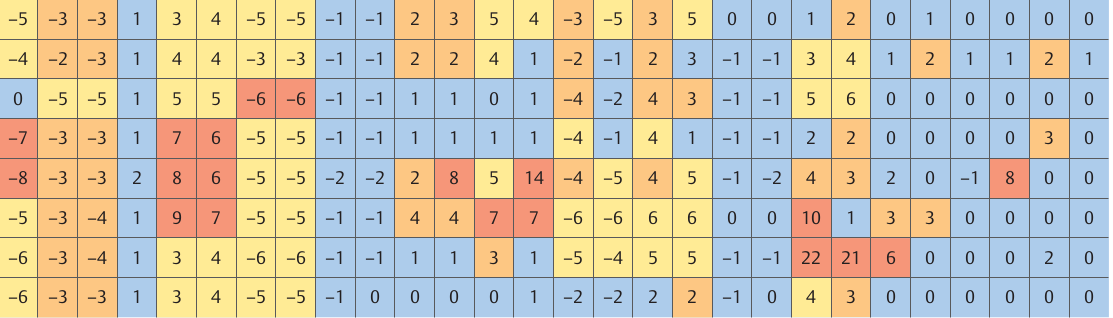
\includegraphics[width=\linewidth]{zmatrix.png}
    \caption{Visualization of the SMPL human body model}
    \label{fig:smpl}
\end{figure}

\subsection{Pose Dictionary}

This approach represents the pose as a combination of known poses. The dictionary of known basis poses can be gather statistically from a 3D pose dataset using techniques like PCA. The matching can be done using an optimization framework  \parencite{ramakrishna2012reconstructing}, \parencite{zhou20153d} or more recently with the help of a Deep Learning model \parencite{zhou2016sparseness}, \parencite{chen20173d}, \parencite{tome2017lifting}. This methodology has the drawback that each pose can be represented in multiple ways and can lead to invalid 3D poses. This can be mitigated by jointly optimizing a pose matching and joint angle limit constraints \parencite{akhter2015pose}.

\subsection{Model-free}

Regressing the joint positions directly has become more popular in the recent work which use Deep Learning models , \parencite{pavlakos2017coarse}, \parencite{martinez2017simple}, \parencite{hossain2017exploiting}, \parencite{tekin2017learning}. These methods are much more simple in the pose representation and rely on the Deep Learning models to learn the structural information in the human body. One downside of this methods is the lack of structural priors can lead the model to make anthropometrically invalid 3D pose estimations.

\section{2D Pose Estimation}

Since our solution pipeline starts with estimating 2D poses from monocular images we will discuss the prominent techniques in this area. 2D pose estimation aims to localize certain number of joints in the image. This information although ambiguous on its own can be used in later stages to estimate the full 3D pose of the person.

One of the most prominent results in 2D pose estimation have been obtained by Newell et. at \parencite{newell2016stacked}. He uses repeated top-down and bottom-up processing steps in conjunction with intermediate supervision to achieve very strong results. Each block in the network is called hourglass and consists of encoding and decoding layers. Each hourglasses are stacked on top of each other and refine each other's output. The whole architecture is trained end-to-end.

Many methods build on top of the Stacked Hourglass model. \parencite{chu2017multi} use Conditional Random Fields to associate neighboring regions and body part attention model to impose global consistency of the body. \parencite{chou2017self} uses adversarial training to give a meaningful structural priors for the body poses. The discriminator helps the model reject invalid joints angles and anthropometrically invalid poses.

\parencite{iqbal2017posetrack} and \parencite{insafutdinov2017arttrack} attempted estimating the pose for multiple people in  videos. Both approaches are closely related but differ in the type of body-part proposals and the structure of the spatio-temporal graph where Iqbal et. al. rely on \parencite{insafutdinov2016deepercut} for body-part detectors Insafutdinov et. al. use person-conditioned model that is trained to associate body parts of a specific person already at the detection stage. 

\parencite{cao2016realtime} utilized a CNN based model similar to the Stacked Hourglass model where they refine their predictions in multiple steps. They added another branch to the model which predicts Part Affinity Fields (PAFs). This enables multi-person pose estimation by predicting association fields between joints. PAFs are later used to match the joints in a bottom-up process. This algorithm can run in real-time on commodity hardware.

\section{3D Pose Estimation}

There are many different approaches to 3D human pose estimations. Recently some methods use Deep Neural Networks to estimate the 3D pose directly from images \parencite{pavlakos2017coarse}, \parencite{tekin2016structured}, \parencite{varol2017learning}, \parencite{rogez2016mocap}. Some models have tried to formulate the problem as a retrieval task. Similar poses are searched from a dictionary and then combined or refined to get the final pose []. Another line of research uses either ground truth 2D poses or estimates from a 2D pose estimator to train a model that lifts the 2D poses to 3D. Other methods use additional information besides the given image like temporal information [] or structural priors []. We will discuss these methods in more detail below.

\subsection{Deep network trained end-to-end}

The emergence of the Human3.6M \parencite{ionescu2014human3} enabled the use of end-to-end trained Deep Learning models to estimate 3D human poses directly from images. Although these methods rely on a laboratory setup which doesn't generalize well to the in-the-wild scenes algorithmic innovation has shown many advances. The Human3.6M database benchmark has been constantly improving ever since.

Pavlakos et al. \parencite{pavlakos2017coarse} predicts volumetric heat maps for the joints and uses an iterative refinement strategy to improve the heat maps. Tekin et. al. \parencite{tekin2016structured} try to solce the problem of anthropometrically invalid poses by training a de-noising auto-encoder to encode the human pose in an embedding. The auto-encoder is stacked on top of a Convolutional Neural Network and later fine tuned together end-to-end.

Another line of research focuses of synthesizing novel frames by augmentation. Varol et. al. \parencite{varol2017learning} showed that learning from synthetic scenes can be effective in especially when combined with real scenes to predict depth and body segmentation. \parencite{rogez2016mocap} generated synthetic images by blending real images  together and showed that this techniques improves prediction accuracy.

Following sections show methods which improve the direct estimation methods by utilizing combined training of 2D and 3D poses, temporal information or structural priors.

\subsection{Pose Dictionaries}

Some approaches utilize a 3D pose dictionary to look up similar poses. This can take the form of an embedding or collection of joint positions which are then refined using an optimization mechanism.

Rogez et. al. \parencite{rogez2017lcr} build an anchor-pose dictionary by clustering a subset of the training images. A region proposal network \parencite{ren2015faster} outputs anchor-pose proposals given an image. Another network scores the anchor-poses in one branch by a classification loss and refines them in another branch using a regression loss. Finally the refined and scored anchor poses are integrated to give the 3D pose estimate.

Zhou et. al. \parencite{zhou2016sparseness} use a Convolutional Neural Network to estimate a sequence of joint heat maps and use the Expectation-Maximization algorithm to estimate the 3D pose out of a 3D pose dictionary. 

In \parencite{chen20173d} Chen et. al. assume the conditional independence of 3D pose from the image given the 2D pose. This makes their solution a 2 part solution. They estimate the 2D pose with a Convolutional Neural Network and use a Non-parametric Nearest Neighbor model to match the 2D pose to a known 3D pose. 

The accuracy of these models depend on the size of the Pose Dictionary. No matter how large the pose dictionary there will be still unobserved poses on the tail end of the pose distribution. This makes making inference and finding a large enough dictionary prohibitively expensive.

\subsection{2D Information}

2D Pose estimation has seen incredible progress in recent years \parencite{cao2016realtime}, \parencite{newell2016stacked}, \parencite{iqbal2017posetrack}. 2D pose estimation is a necessary part of 3D pose estimation which lead many researches to either use 2D pose estimation as an additional supervision signal or decouple the two problems and use the 2D poses as input to the 3D pose estimation problem. Both methods have shown remarkable improvements over the baseline since they can effectively utilize the abundant 2D pose datasets. 

Park et. al. \parencite{park20163d} used a Deep Learning model which estimates both 2D and 3D pose. While the 3D pose estimation is formulated as a regression problem the 2D pose estimation is formulated as a classification problem where the image is tiled into grids and each joint is classified to one grid. The search space for 3D pose is much larger which prevents the use of the grid tiling. The network has a Convolutional Neural Network architecture where it branches out in the fully connected layers into two parts. The 3D joint locations are predicted by combining multiple candidate poses which act as an ensemble mechanism. Zhou et. al. \parencite{zhou2017towards} use a Convolutional Neural Network architecture  similar to \parencite{newell2016stacked} which estimates 2D pose of joints with a Depth Regression module in the end. During training both 2D and 3D pose datasets are mixed. For 3D pose examples Euclidean Loss for joint errors is applied and for 2D pose examples a weakly supervised loss is applied which depends on 2D annontaitons and human skeletal priors.     

Tekin et. al. \parencite{tekin2017learning} use a Convolutional Neural Network to estimate 2D confidence maps for each joint. Those confidence maps and the original image are fed into 2 branches of a Convolutional Neural Network and their feature maps are fused together to estimate the final 3D pose. A similar mechanism is performed by Tome et. al. \parencite{tome2017lifting}. Their approaches differ mainly in that Tome et. al. don't separate 2D pose estimation to a separate branch. They use a iterative refining mechanism similar how \parencite{newell2016stacked} used where in each stage they predict 2D confidence maps for the joints, estimate 3D pose from those, project the 3D pose into 2D and fuse the projected 2D pose estimate with the 2D confidence map and apply a re-projection error. After the iterative refinement the lifting operation which gives the final 3D pose. Nie et. al. \parencite{nie2017monocular} train 2 networks separately a Skeleton Long-Short Term Memory Network \parencite{hochreiter1997long} which estimates global 3D pose given 2D pose and a Patch Long-Short Term Memory Network which given image patches around the joints estimates the depth of those joints. The two network are later integrated in the second layer Long-Short Term Memory Network by combining the output of the two and estimating the depth of the joints. The architecture has a multi-task with depth prediction loss and 2D pose estimation loss which enables the use of in-the-wild 2D pose databases. 

Moreno et. al. \parencite{moreno20173d} use the output of a off-the-shelf 2D pose detector as input. This has the advantage of profoundly simplifying the estimation process. First they compute the Euclidean Distance Matrix (EDM) which encodes the distances between each joint. The EDM is fed into a Convolutional Neural Network which estimates a Euclidean Distance Matrix for 3D pose. This is used to predict the 3D joint locations using Multidimensional Scaling. Martinez et. al. \parencite{martinez2017simple} follow a similar approach where they use the output of a off-the-shelf 2D pose detector. They train a simple 4 layer feed-forward neural network with residual connections to lift the 2D pose into 3D. This simplifies the training procedure immensely without loosing the accuracy benefits and enables them to accurately estimate the pose in images which are visually demanding.

\subsection{Temporal Information}

3D pose estimation when done without considering the temporal context can be noisy. The source of the noise can be occlusions inherent randomness in the model which cause its estimations to become jittery and occasional missing joints. A solution to this problem is to use the video as the input and estimate 3D pose sequences. The temporal consistency constraint results in an estimation that is smooth and doesn't contain missing joints since they will be interpolated by the network. Another benefit of using temporal information is the fact that certain ambiguities can be removed by utilizing the fact that the size of the skeleton of the person doesn't change during the sequence. This helps the network interpret change in apparent size as the person becoming closer to the camera.

Lin et. al. \parencite{lin2017recurrent} utilize an iterative refinement mechanism using Long-Short Term Memory Networks (LSTM) \parencite{hochreiter1997long}. This enables them to both utilize temporal information and use the critical refinement strategy which many of the state-of-the-art methods rely on heavily. They designed their architecture in stages to enable refinement where the 2D pose estimation module and 3D pose module give their outputs to the next stage receive outputs from the previous one. Inside each stage the 2D pose module which estimates image dependent pose representations given the previous stages output and the image . The feature maps are then passed to bot the next stage through constitutional filters and the feature adaptation module which lifts the feature maps to 3d and passed them to 3D pose module. 3D pose module estimate the 3D pose given the previous pose estimate and the feature adaptation modules output and passes the pose estimate to the next stage.

Hossain et. al. \parencite{hossain2017exploiting}, \parencite{hossain2017understanding} extended \parencite{martinez2017simple}'s work by exploiting temporal information through a sequence-to-sequence architecture similar to \parencite{sutskever2014sequence}. Their model is much simpler than their counterparts \parencite{lin2017recurrent}, \parencite{bogo2016keep}, \parencite{mehta2017vnect} which utilize temporal information thanks to the fact that they use 2D poses from an off-the-shelf 2D pose detector. This boils the problem down to lifting the pose to 3D.

\subsection{Structural Priors}

3D pose estimation is an ill-posed problem since the 2D projection of a 3D pose is not unique. If we assume that there are 17 joints in the body as it is depicted in the Human3.6M dataset \parencite{ionescu2014human3} there are 51 data points that we need to estimate to get a 3D pose. However, the set of 2D joint locations contain 34 data points. So in one sense we have more unknowns than constraints. Fundamentally this can be thought as the source of the ambiguity. One approach to counteract this ambiguity it to introduce additional constraints which relate to the skeletal structure. Some of the known qualities of the human skeleton are:
\begin{itemize}
    \item Some key-points in the human body like joints are connected with bones whose length is constant throughout a pose sequence
    \item Bone lengths adhere to the anthropometric proportions, which can be statistically estimated.
    \item There are limits to the degree of freedom that some joints have, like the knee and elbow joints.
    \item There are limits to the amount each joint can rotate.
    \item Some key points in the human body are on the same bone structure and act as parts of a rigid body. Like eyes, ears, nose, top of the head which all locate on the head and move together.
    \item Human body has a left-right symmetry. This means bone lengths of the left side of the body are the same to the bone lengths in the right side of the body.
\end{itemize}

All these qualities act as additional constraints to the 3D pose estimation problem. Considering these properties can aid in estimating valid and plausible 3D poses.

Earlier work \parencite{barron2001estimating}, \parencite{wei2009modeling} used these constraint in an optimization framework to estimate the 3D pose given 2D joint positions. More recently Zhou et. al. \parencite{zhou2016deep} used a differentiable kinematic object model to represent the human pose. They used a standard Convolutional Neural Network to estimate motion parameters which are fed to a kinematic layer which estimates joint locations. Since the kinematic transformation is differentiable the whole model is trained end-to-end. They show that using a kinematic model gives 4,7\% reduction in average joint error. A similar approach was developed by Fang et. al. \parencite{fang2018learning} where they used known relations between joints called Pose Grammars namely Symmetry Grammar which enforces the left and right sides of the body are symmetric, Kinematic Grammar which incorporates kinematic relation between joints and Motor Coordination Grammar which enforces locomotion patterns between the right and left side of the body. They use 2D joint positions as input similar to Martinez et. al. \parencite{martinez2017simple} and use Bidirectional Recurrent Neural Networks \parencite{schuster1997bidirectional} to model grammars. Show that this constrains improve the prediction accuracy by a large margin. Sun et. al. \parencite{sun2017compositional} re-parametrize the pose representation to take the bones into the center. Traditionally the human body is represented as a set of joints where the hip joint is located at the origin and all other joints are located with respect to the hip joint. They organize the joints in a tree like fashion where each joint has only one parent but can have multiple children. The bone corresponding to a joint is defined based on the parent's position. This compositionality is also reflected in the loss function. They show that by defining the loss as the relationship between all joint pairs they can effectively model the skeletal structure and reduce the per joint error. 

Another approach to skeleton modeling is using Deep Netorks to train an embedding that represents the manifold of valid poses. Chen et. al. \parencite{chen2017adversarial} used a Generative Adversarial Networks \parencite{goodfellow2014generative} to build the skeleton embedding. This is achieved by adding a Pose Discriminator which discriminates against invalid poses and a Confidence Discriminator which helps the model predict joint positions with higher confidence. 

SMPL \parencite{loper2015smpl} is a statistical human body model which is parameterized both in terms of the kinematic relation between joints and the shape of the person. Bogo et. al. \parencite{bogo2016keep} use the DeepCut \parencite{pishchulin2016deepcut} model to estimate the 2D joints positions and fit the SMPL body model using an optimization mechanism which minimizes re-projection loss for the joints, shape priors, joint angle priors and pose priors. Huang et. al. extend this work \parencite{huang2017towards} by fitting the 3D pose to 2D joints detected from multi-view images, fit the 3D body model to the contours produced by a Convolutional Neural Network and utilize a Discrete Cosine Transform (DCT) \parencite{akhter2012bilinear} temporal prior. This results in a drastic improvement over their baseline. Kanazawa et. al. \parencite{kanazawa2017end} used the SMPL model in a Deep Learning architecture. They use a Convolutional Neural Network to estimate camera parameters, 3D pose parameters, and shape parameters. The shape parameters and 3D pose parameters are used in the SMPL model to generate a human pose. Adversarial training is being performed where the the discriminator helps the model learn a manifold of valid shapes. The pose is projected back to the 2D frame using the camera parameters and re-projection loss is applied to the joints. This approach enables the training for lifting to a 3D pose without a 3D annotated dataset and instead use visually much more diverse and large 2D pose datasets. 3D pose datasets are used to learn skeletal structure using adversarial training.   

Mehta et. al. \parencite{mehta2017vnect} use a combination of Bounding box tracking, a 2D confidence map and 3D joint position estimation, temporal regularization and skeletal fitting to train a deep convolutional neural network. Their architecture is general where they can estimate poses in multi-person scenes with temporal smoothing however they only rely on Human3.6M and MPII-3D-INF datasets to train which results in poorer accuracy than their counterparts using similar techniques. They extended their previous work \parencite{mehta2017single} by incorporating Part Affinity Fields \parencite{cao2016realtime} and Occlusion Robust Location Maps (ORLM). They also employ a training procedure where they train on 2D dataset by freezing the 3D pose estimation branch of their network and train on a separate 3D pose dataset to learn 3D mapping.

Debral et. al. \parencite{dabral2017structure} use the stacked hourglass \parencite{newell2016stacked} model for 2D pose estimations. They first train the 2D pose model separately. Later they stack a 3D pose estimator on top of the stacked hourglass. Then they add structural consistency losses like symmetry loss and illegal angle loss. Lastly, they train a separate RNN model which smooths out the 3D pose estimations.
